\section{Funções de Duas Variáveis}

	\subsection{Definição \cite{morettin}}

		Seja $D$ um subconjunto do $\mathbb{R}^{2}$. Chama-se função de $D$ em $\mathbb{R}$ toda relação que associa a cada par ordenado $(x, y)$ pertencente a $D$ um único número real indicado por $f(x, y)$. O conjunto $D$ é chamado domínio da função e $f(x, y)$ é chamado de imagem de $(x, y)$ ou valor de $f$ em $(x, y)$.

	\subsection{A Função de Cobb-Douglas \cite{morettin}}

		A função de Cobb-Douglas relaciona a quantidade produzida de algum bem em certo intervalo de tempo com os insumos variáveis necessários a essa produção (trabalho, terra, capital e outros). Um modelo de função de produção muito utilizado foi introduzido pelo economista Paul Douglas e pelo matemático Charles Cobb, ambos norte-americanos, em seus estudos sobre a repartição da renda entre o capital e o trabalho no início do século XX. A expressão da referida função é

		\bigskip

		{\LARGE $P = f(L, K) = A \times K^{\alpha} \times L^{1 - \alpha}$} ,

		\bigskip

		em que

		\textbf{$P$} é a quantidade produzida, \\
		\textbf{$K$} é o capital empregado, \\
		\textbf{$L$} é a quantidade de trabalho envolvido.

		A constante \textbf{$A$} depende da tecnologia utilizada e \textbf{$\alpha$}  é um parâmetro que varia de $0$ a $1$.

	\subsection{Gráficos de Funções de Duas Variáveis \cite{morettin}}

		Vimos, no estudo de funções de uma variável, que seu gráfico era o conjunto

		\bigskip

		{\LARGE $\{(x, y) \in \mathbb{R}^{2} \mid y = f(x) \ \text{e} \ x \in D\}$} .

		\bigskip

		Consequentemente, a representação gráfica era feita no plano cartesiano (Figura 9.2).

		\begin{figure}[H]
			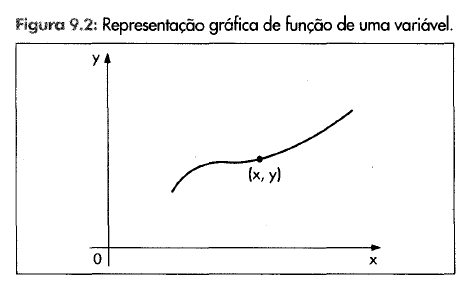
\includegraphics[height=6.5cm]{images/morettin_figura-9-2}
		\end{figure}

		De modo totalmente análogo, definimos o gráfico de uma função de duas variáveis. Seja $f(x, y)$ uma função de duas variáveis $x$ e $y$. O gráfico da função é o conjunto

		\bigskip

		{\LARGE $\{(x, y, z) \in \mathbb{R}^{3} \mid z = f(x, y) \ \text{e} \ (x, y) \in D\}$} .

		\bigskip

		Portanto o gráfico de $f(x, y)$ será representado no espaço tridimensional, de tal forma que a cada par $(x, y)$ do domínio corresponda uma cota $z = f(x, y)$, como mostra a Figura 9.3.

		\begin{figure}[H]
			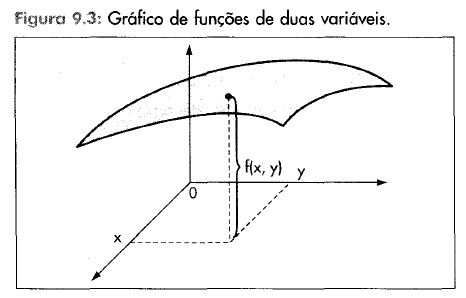
\includegraphics[height=6.5cm]{images/morettin_figura-9-3}
		\end{figure}
		
			\subsection{Curvas de Nível \cite{morettin}}

		Devido à dificuldade de desenharmos o gráfico de uma função de duas variáveis, costumamos utilizar a seguinte forma alternativa de representação: obtemos o conjunto dos pontos do domínio que têm a mesma cota $c$; tais pontos, em geral, formam uma curva que recebe o nome de curva de nível $c$ da função (Figura 9.14)

		\begin{figure}[H]
			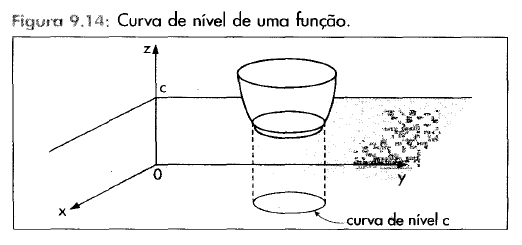
\includegraphics[height=5.5cm]{images/morettin_figura-9-14}
		\end{figure}

		Assim sendo, atribuindo valores a $c$, obtemos várias curvas de nível, que permitem tirar importantes informações sobre a função.

		O método das curvas de nível, além de ser muito utilizado em Economia, é também utilizado em outras áreas, como Engenharia (topografia de terrenos), Geografia e outras.

		\bigskip

		\textbf{Exemplo 9.9}. Seja a função $f(x, y) = x^{2} + y^{2}$. As curvas de nível $c = 1$, $c = 2$ e $c = 4$ são:

		\bigskip

		$c = 1 \Rightarrow x^{2} + y^{2} = 1$ (circunferência de centro $(0, 0)$ e raio $1$), \\
		$c = 2 \Rightarrow x^{2} + y^{2} = 2$ (circunferência de centro $(0, 0)$ e raio $\sqrt{2}$), \\
		$c = 3 \Rightarrow x^{2} + y^{2} = 4$ (circunferência de centro $(0, 0)$ e raio $2$).

		\bigskip

		Essas curvas de nível aparecem na Figura 9.15.

		\begin{figure}[H]
			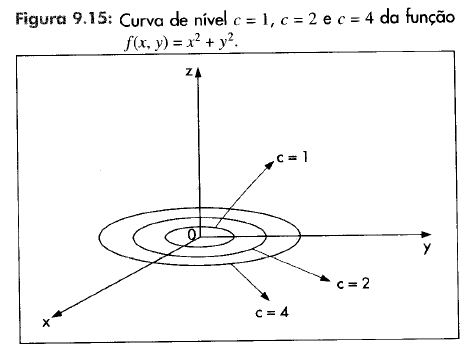
\includegraphics[height=7cm]{images/morettin_figura-9-15}
		\end{figure}

		Frequentemente, a representação das curvas de nível é feita desenhando-se apenas os eixos $0x$ e $0y$, como na Figura 9.16.


		\begin{figure}[H]
			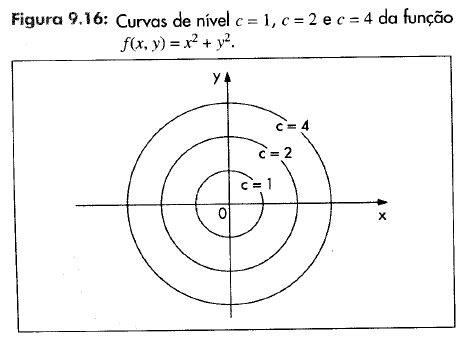
\includegraphics[height=7cm]{images/morettin_figura-9-16}
		\end{figure}
		
		\subsubsection{Curvas de Isoproduto ou Isoquantas de Produção \cite{morettin}}

			Consideremos a função de produção $P = L^{0,5} \times K^{0,5}$, em que $L$ representa o trabalho envolvido e $K$, o capital.

			As cuvas de nível $c = 1$ e $c = 2$ são:

			\medskip

			$c = 1 \Rightarrow L^{0,5} \times K^{0,5} = 1 \Rightarrow L = \cfrac{1}{K}$, \\
			$c = 2 \Rightarrow L^{0,5} \times K^{0,5} = 2 \Rightarrow L = \cfrac{4}{K}$ .

			\medskip

			A representação dessas curvas de nível comparece na Figura 9.17. Cada curva de nível fornece os pares $(K, L)$ para os quais a produção é constante, sendo a primeira com produção igual a $1$ e a segunda igual a $2$. Em Economia, essas curvas de nível são denominadas \textbf{curvas de isoproduto} ou \textbf{isoquantas de produção}.

			\begin{figure}[H]
				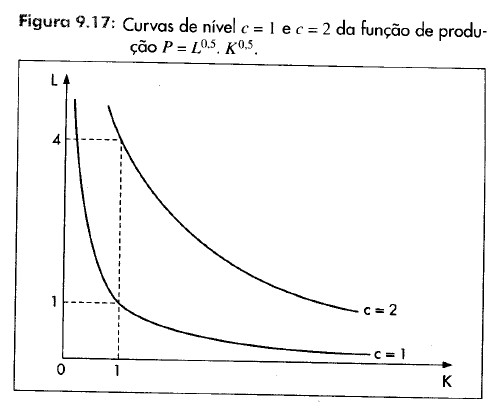
\includegraphics[height=7.5cm]{images/morettin_figura-9-17}
			\end{figure}
			
	\subsection{Limite e Continuidade \cite{morettin}}

		As noções de limite e continuidade para funções de duas variáveis são análogas às que foram vistas para funções de uma variável.

		Intuitivamente falando, o limite de $f(x, y)$ quando $(x, y)$ tende ao ponto $(x_{0}, y_{0})$ é o número $L$ (se existir) do qual se aproxima $f(x, y)$ quando $(x, y)$ se aproxima de $(x_{0}, y_{0})$, por qualquer caminho, sem no entanto ficar igual a $(x_{0}, y_{0})$.

		Indicamos essa ideia da seguinte forma:

		\bigskip

		{\LARGE $\lim \limits_{(x, y) \to (x_{0}, y_{0})} f(x, y) = L$} .

		\bigskip

		Caso $L$ seja igual a $f(x_{0}, y_{0})$, dizemos que $f$ é contínua em $(x_{0}, y_{0})$; caso contrário, $f$ é dita descontínua em $(x_{0}, y_{0})$.
		
		\subsubsection{Teorema 1 \cite{morettin}}

			São contínuas em todos os pontos de seu domínio as funções:

			\begin{enumerate}[label=(\alph*)]

				\item Polinomiais nas variáveis $x$ e $y$ ;
				\item Racionais nas variáveis $x$ e $y$ .

			\end{enumerate}

			Assim, de acordo com o Teorema 1, são contínuas por exemplo, as funções:

			\bigskip

			$f(x, y) = x^{2} + y^{2} - xy, \forall x, y$ (polinomial), \\
			$f(x, y) = x^{3}y^{2} - xy + y^{3} +6, \forall x, y$ (polinomial), \\
			$f(x, y) = \cfrac{x^{2} + y^{2}}{xy - 1}, \forall x, y \ \text{tais que} \ xy \neq 1$ (racional).
			
		\subsubsection{Teorema 2 \cite{morettin}}

			Se $f(x, y)$ e $g(x, y)$ são contínuas em $(x_{0}, y_{0})$, então serão também contínuas em $(x_{0}, y_{0})$ as funções:

			\begin{enumerate}[label=(\alph*)]

				\item $f(x, y) + g(x, y)$
				\item $f(x, y) - g(x, y)$
				\item $k \times f(x, y) \ \ (k \in \mathbb{R})$
				\item $f(x, y) \times g(x, y)$
				\item $\cfrac{f(x, y)}{g(x, y)} \ \ (g(x_{0}, y_{0}) \neq 0)$
				\item $a^{f(x, y)} \ \ (a > 0)$
				\item $\log f(x, y) \ \ (f(x_{0}, y_{0}) > 0)$
				\item $\cos f(x, y)$
				\item $\sin f(x, y)$

			\end{enumerate}

			De acordo com os teoremas vistos, são contínuas em todos os pontos de seu domínio, por exemplo, as funções:

			$f(x, y) = x^{2} + y^{2} - 2xy^{3}$ ,\\
			$f(x, y) = \cfrac{x + y}{x - y}$ ,\\
			$f(x, y) = 2^{x - y^{2}}$ ,\\
			$f(x, y) = \ln (x + y)$ ,\\
			$f(x, y) = \sin (x^{2} + y)$ ,\\
			$f(x, y) = x^{2} + e^{x}$ .